\documentclass{beamer}
\usepackage[latin1, utf8]{inputenc}
\usepackage[francais]{babel}
\usepackage{wrapfig}
\usepackage{framed}
%****
\usepackage{multimedia}
%\usepackage{media9}
\usepackage{hyperref}

\useoutertheme[height=0pt,left]{sidebar}
\usecolortheme{seahorse}
\setbeamercolor*{titlelike}{parent=structure}
\useinnertheme{circles}
\setbeamertemplate{frametitle}[default][right]

%\title{Les robots ressemblant à l'humain sont-ils vraiment utiles ?}
\title{\textsc{L'imitation de l'être humain}}
\author{Christian LASSERRE \& Théophile GUILBAUD}
%\institute{ENSEIRB-MATMECA}
\date{}

\begin{document}
\begin{frame}
  \titlepage
  {
    \vspace*{-1cm}
    \begin{center} 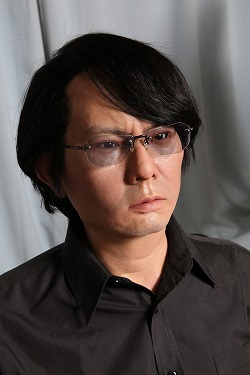
\includegraphics[width=40mm]{data/HI-4} \end{center}
  }
\end{frame}

\begin{frame}
  \tableofcontents
\end{frame}

\section{Ressemblance}
\begin{frame}{RESSEMBLANCE}
  ``Quel rôle joue l’imitation la culture et quelle est son importance pour le savoir anthropologique ? Ce texte souligne quelques voies d’approche possibles. L’imitation peut être envisagée comme une stratégie parodique, une compétence cognitive, un moyen de \colorbox{yellow}{transmission culturelle}, un principe de l’\colorbox{yellow}{apprentissage social} ou un \colorbox{yellow}{mécanisme d’adaptation}. Les processus d’imitation impliquent des \colorbox{pink}{compétences cognitives spécifiques} et s’inscrivent dans des \colorbox{pink}{contextes sociaux et culturels déterminés}. Parce qu’ils se situent à la charnière des sphères du biologique et du culturel, ces processus font partie du projet anthropologique qui cherche à comprendre à la fois l’unité cognitive de l’homme et la diversité de ses réalisations culturelles.''
  ~\\~\\
  {\small Nélia Dias, dans ``Imitation et Anthropologie''}
  
\end{frame}

\subsection{Le(s) Géminoide(s)}
\begin{frame}{Histoire}
  Professeur
\end{frame}

\begin{frame}{Auteur}
\end{frame}

\subsection{Caractéristiques}
\begin{frame}{Geminoide HI-4}
  \begin{framed}
    \begin{wrapfigure}{l}{40mm}
      \centering
      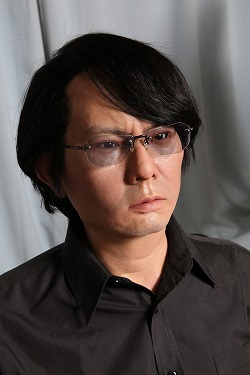
\includegraphics[width=40mm]{data/HI-4}
      \caption{Geminoïde HI-4}
    \end{wrapfigure}
    Il était une fois ...
  \end{framed}
\end{frame}

\begin{frame}{Geminoide HI-2}
\end{frame}

\begin{frame}{Geminoide F}
  (il y a aussi le DK...)
  convention social -> uniquement physique
\end{frame}

\subsection{Conclusion}
\begin{frame}{ça ressemble à un humain}
\end{frame}

\section{L'intéraction}
\begin{frame}{INTERACTIONS}
  \begin{figure}
    \centering
    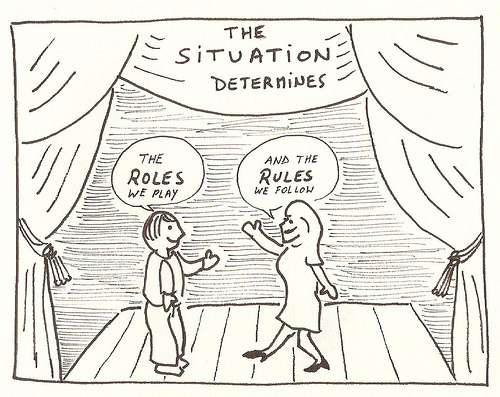
\includegraphics[width=\textwidth]{data/interaction}
    \caption{Le robot Telenoide}
  \end{figure}
\end{frame}

\subsection{Télénoïde}
\begin{frame}{Présentation}
  \begin{figure}
    \centering
    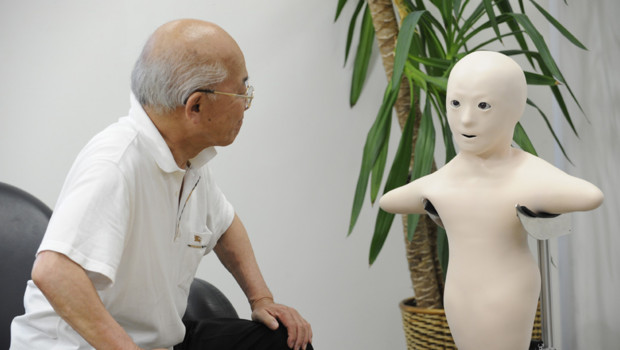
\includegraphics[width=50mm]{data/telenoid}
    \caption{Le robot Telenoide}
  \end{figure}
  Le robot qui transfère votre présence
\end{frame}

\begin{frame}{Caractéristiques}
  \begin{itemize}
  \item 7 versions (depuis aout 2010)
  \item taille : 50cm
  \item poids : 3.5kg
  \item capteurs : 2 microphones
  \item alimentation : batterie
  \item degré de liberté
    \begin{itemize}
    \item 3 sur les yeux
    \item 1 sur la bouche
    \item 3 sur le coup
    \item 2 sur les moignons
    \end{itemize}
  \item peau en PVC
  \item prix 35.000\$ les premiers (environ 8.000\$ desormais)
  \end{itemize}
\end{frame}

\subsection{Utilité}
\begin{frame}
  Design androgyne pour permettre la diversité des utilisateurs.
  \\~\\
  Pas encore assez de capteurs.
  \\~\\
  C'est un téléphone qui a pour but de retransmettre l'idée présence.
  \\
  \begin{itemize}
  \item accueil hotel/aéroport
  \item sex-symbol
  \item ...
  \end{itemize}
\end{frame}

\begin{frame}{Avenir}
  Le robot qui nous permettra l'ubiquité\\
  %\movie[showcontrols]{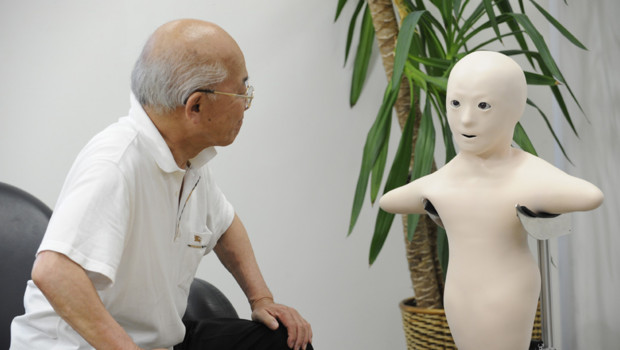
\includegraphics[width=0.8\textwidth]{data/telenoid}}{data/Telenoid_in_action.mp4}
  %\movie[label=cells,width=4cm,height=3cm,poster,showcontrols,duration=5s]{}{data/Telenoid_in_action.mp4}
  %(\href{run:mplayer data/Telenoid_in_action.mp4}{VIDEO})
  \movie[label=cells,width=4cm,height=3cm,externalviewer,showcontrols]{VIDEO}{data/Telenoid_in_action.mp4}
\end{frame}

\subsection{Conclusion}
\begin{frame}
  Robot Inhabituel, contre exemple de ce qu'on attend d'un robot.
  Aucune étude de proxémie, convention sociale développée, etc...
\end{frame}

\end{document}
